%% paper.tex
%% V1.4b
%% 2017/03/05
%% by HSNL, NTHU


\documentclass[journal]{IEEEtran}

\usepackage{graphicx}
\usepackage{indentfirst}
\usepackage{cite}
\usepackage{url}
\usepackage{hyperref}
\usepackage{amsmath}
\usepackage{enumerate}
\usepackage[flushleft]{threeparttable}
\usepackage[super]{nth}


\begin{document}


\title{Performance Optimization of Service Chain for vCPE in Small Networks with OpenFlow Switch}

% author names and IEEE memberships
\author{\IEEEauthorblockN{
Nen-Fu Huang\IEEEauthorrefmark{1},
Chia-An Lee\IEEEauthorrefmark{1},
Chi-Hsuan Li\IEEEauthorrefmark{1},
Chia-Chi Chen\IEEEauthorrefmark{1},
I-Hsien Hsu\IEEEauthorrefmark{1}, \\
Che-Chuan Li\IEEEauthorrefmark{1},
Ching-Hsuan Chen\IEEEauthorrefmark{2} and
I-Ju Liao\IEEEauthorrefmark{1}}

\IEEEauthorblockA{
\IEEEauthorrefmark{1}
Department of Computer Science National Tsing Hua University, Hsinchu, Taiwan} \\
\IEEEauthorblockA{
\IEEEauthorrefmark{2}
Institute of Communication Engineering National Tsing Hua University, Hsinchu, Taiwan}
}

% The paper headers
% \markboth{Journal of \LaTeX\ Class Files,~Vol.~14, No.~8, August~2015}%
% {Shell \MakeLowercase{\textit{et al.}}: Bare Demo of IEEEtran.cls for IEEE Journals}

% make the title area
\maketitle


\begin{abstract}
In the last decade, along with the continuously developing of software defined network (SDN), numerous SDN applications have played important roles in modern network. Virtual Customer Premise Equipment (vCPE) is one of potential applications can make game change because it can reduce OPEX and CAPEX in the same time. This service compose of many technologies with complex architecture like Virtualized Network Functions (VNFs) and Service Chaining. Many researches discuss algorithm or mechanism to link multiple VNFs as a single Network Function Virtualization (NFV) then connect NFVs as a service chain in cloud. Nevertheless, the hardware resource and characteristic of SDN switch that never mention before may waste in this architecture. In this paper, a vCPE framework with multiple flow table management based on cloud is implemented. The proposed of vCPE framework is to create a SDN-enabled VNF using both resources in SDN switch and on cloud and these VNFs can be deployed as edge. The system is also integrated with an application identification engine based on machine learning algorithms thus providing flow control in vCPE framework with confidence. Experimental results show that the framework provide performance in VNF compete over single table SDN application.
\end{abstract}

% Note that keywords are not normally used for peerreview papers.
\begin{IEEEkeywords}
Software defined network, network function virtualization, NFV orchestration, virtual customer premise equipment, OpenFlow, multiple flow tables
\end{IEEEkeywords}

\IEEEpeerreviewmaketitle{}


% Introduction
% First paragraph of paper need be big Alhabet
\section{Introduction}
\IEEEPARstart{S}{oftware} Define Network (SDN) \cite{sdn-new-norm}, \cite{sdn-comprehensive} has been developing almost a decade since the first OpenFlow article had be presented in 2008\cite{openflow-campus-network}. OpenFlow\cite{sp:openflow13} gives a brand new viewpoint on network research, and makes innovation on industries. This technology proposed not just a novel architecture but also bring out more methods of flexible traffic engineering. After tons of implementations and researches had been proposed, this architecture exposed some weakness in performance. The main concept of this architecture is separating data plane and control plane that put smart control and multi-path into real world. But legacy hardware design eventually put this perfect design into reality. To achieve high speed packet exchange, ternary content-addressable memory (TCAM) plays an important role in legacy fabric switching. This hardware design speed up the packet switching but it also cause high cost and less size problems.
In the beginning, most of SDN switch used legacy hardware design and just add software API support for temporary solution. The smaller TCAM size comes the less flow control rules but it can keep high performance in packet switching. It brings out inter-datacenter dynamic traffic routing because that scenario doesn’t need much flow entries.
At the same time as SDN was developed, Network Function Virtualization (NFV) \cite{nfvwp,nfv-survey,laptop-sdn} has been introduced by telco operators. Operators want to reduce their cost on maintaining old telco platform which may has been operated in 50 years. To replace the old platform with high maintenance cost, they use virtual machine (VM) based on new computers as solutions. This method can really save a lot of money in maintaining old platform but not all of operators have the same requirement as AT\&T; there is another idea about reducing OPEX and CAPEX in enterprise networks that is Virtual Customer Premise Equipment (vCPE) which was innovated by NEC\cite{nec-vcpe}. vCPE manage network functions on operation side to reduce cost which was deployed on cloud \cite{cloud4nfv}. Although both of technical ideas are perfect, it still address two critical problems. The first one is the lack of hardware support because these ideas need large size of flow tables to achieve multi VNF support. And the other is VM based on cloud may slow down the high speed network exchanging network\cite{nfv-placemet, nfv-placement-model}.
From Pica8\cite{pica8-switch} finished their first OpenFlow switches, there are so many implementation method on a SDN switch. Even Open Network Foundation (ONF)\cite{onf} has a series of testing processes, it can’t shows completely testing result of SDN switch especially performance. Let us take flow entries as example, there are single flow table and multiple flow table architectures much more based on hardware or software. Bandwidth control APIs have been an option in OpenFlow 1.3 but there are many switches still didn’t support these API. Even it did support, there are still at least two implementation methods should be noticed. Meters and per queue show different ways controlling bandwidth not mention to accuracy of bandwidth.
Service chain\cite{service-chain} is another concept with vCPE framework because enterprise will apply a bulk of network services. This technic inherit weakness of SDN switches and vCPE so there is no standard to unified interface to link all services. It’s hard to combine and link all switches and cloud service in such complex situation. Different services on cloud must be working fine with different SDN switches and we believe that’s why most of service chain was implemented in VM on the cloud.

Therefore, the purpose of this paper can be summarized as follows:
\begin{enumerate}
\item To achieve extremely speed of packet exchanging of vCPE in small size network, this study proposed a mechanism to control OpenFlow tables which is in different hardware switches such as Lagopus\cite{lagopus-switch}, Pica8\cite{pica8-switch} and Edgecore\cite{edge-core-switch}. It supports single table and multi-table implementation in different switches and sends status and information message to Ryu controller. This mechanism brings out a novel implementation method of VNF that combine hardware and software operations. It not only makes hardware usage more efficiency but also stays maximum flexibility in NFV deployment.
\item To cover most of NFV framework, this vCPE framework offer a multi cloud management feature. It can working with OpenDaylight\cite{opendaylight} on OpenStack\cite{openstack} and Ryu\cite{web:ryu} on Docker\cite{docker} perfectly. Users can deploy their NFV features in any kind of VM system even in public cloud, and monitor it in same system.
\item To control flows with confidence, an application identification algorithm might be in consideration. The first thing comes out must be Intrusion Detection System (IDS) or Intrusion Prevention System (IPS) but there are 2 major weakness of this two kind of technic. The first is it spends a lot of time to identify connections, and network speed may hang on IPS. The other is it may can’t figure out encryption connections because not all of IDS or IPS have key matching feature. Most of modern cloud applications use HTTPS protocol as basic communication method which makes matter even worse. This study gives an algorithm to identify applications with statistical method with machine learning. The algorithm only use connection ``attributes'' to train an identification models such as packet direction, packet length. Afterward, the algorithm can identify network applications by this model. Even encryption connection can be identified with high accuracy because the algorithm monitor packet in statistical way instead of trying to decode it.
\item To analysis performance of this vCPE framework, this study integrate all of functions mention above to evaluate it compare with the single-table mechanism.
\end{enumerate}

This paper is structured as follows. Section II introduce the overall architecture of the framework what this study proposed. Section III describe multi table management mechanism in the beginning. Rest of section will show how to implement VNF with the mechanism. Section IV considers application identification in SDN because system can do nothing if the system doesn’t know what kind of application running on the network. Section V analytically performance of vCPE framework what we proposed include comparison with traditional network devices. Conclusion and future works will summary in the last section.





\section{System Description}
\subsection{Overview of Network Functions} \label{ssec:desc_nfv_overview}
Our network functions (Fig. \ref{fig:desc_nfv_overview}) are designed with SDN-enabled NFV architecture concept \cite{sdn-enabled}, using the synergies between computer infrastructures (NFVs) and network infrastructures (NFVIs) \cite{nfv2014-v121, nfv2015}.
An NFV is a VNF controller, mainly used for addressing stateful processing and NFVI is an SDN switch used for stateless processing.

\begin{figure}[!t]
\centering
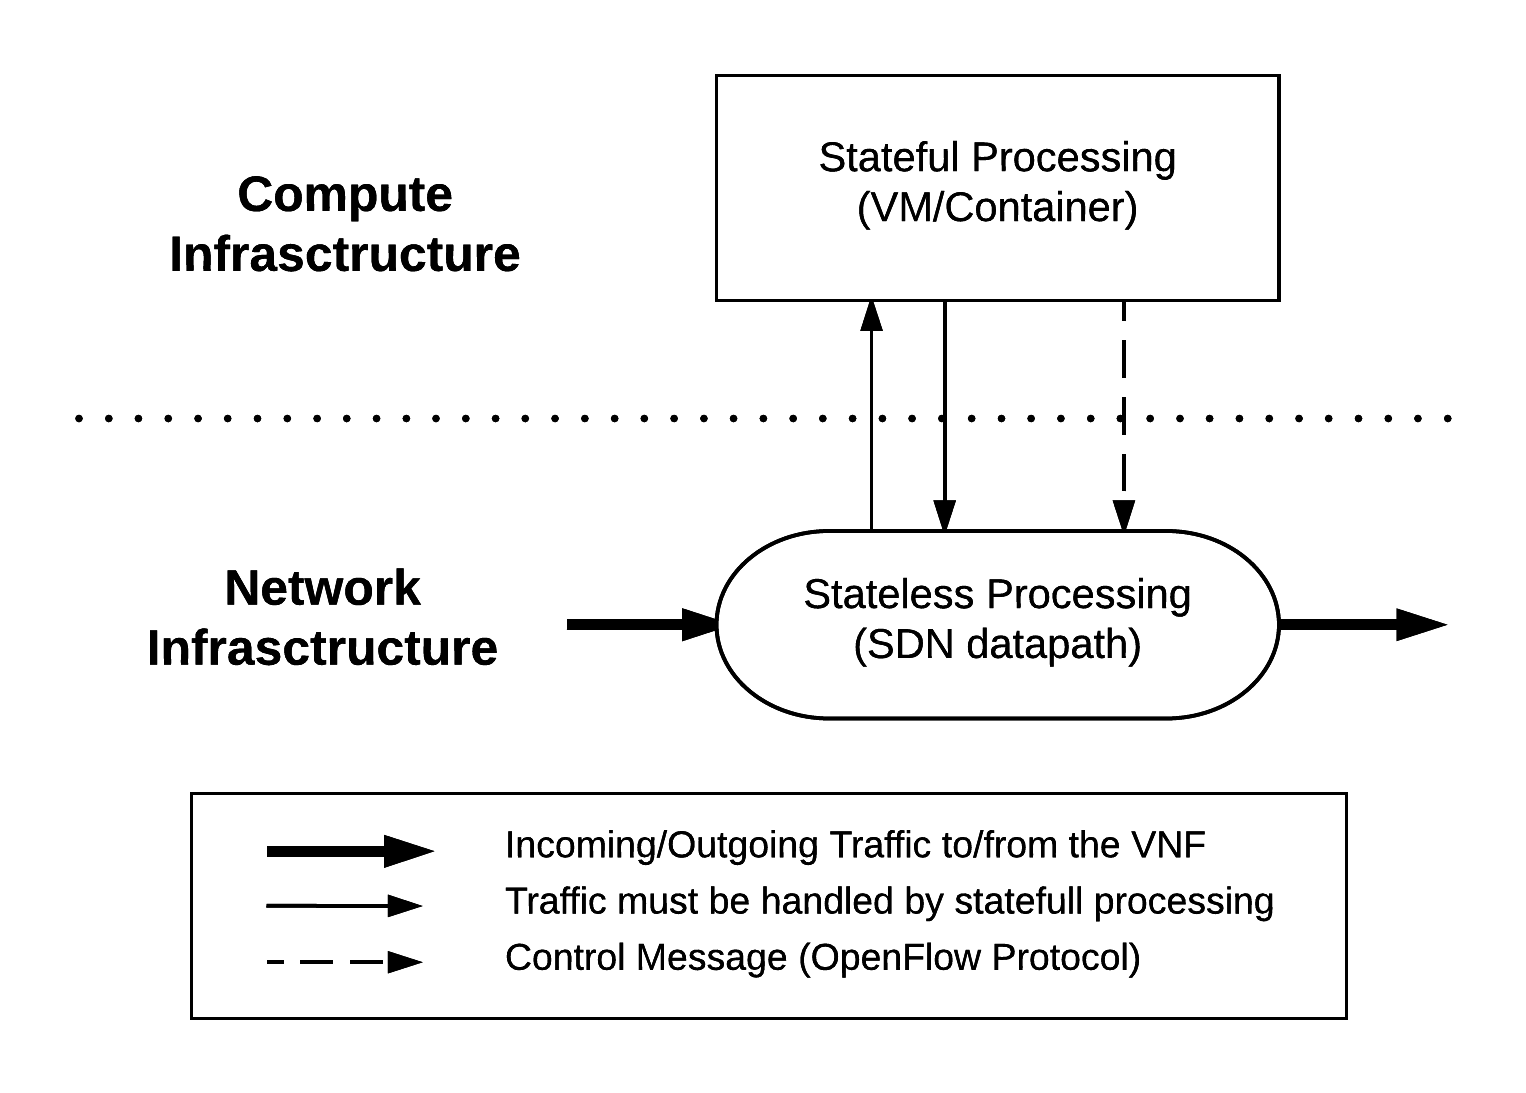
\includegraphics[width=2.5in]{./figures/desc_nfv_overview}
\caption{Overview of network functions.}
\label{fig:desc_nfv_overview}
\end{figure}

\subsubsection{Stateful Processing Component (VNF Controller in VM/Container)}
This component is used to control the workflow, maintain the state associated with the VNF, and provide an interface for service providers or customers to configure and update the behavior of the stateless datapath processing component. We used an SDN controller to implement the VNF controller; and notably, we use southbound APIs of the SDN controller framework to manage the interface between the stateful and stateless components with the OpenFlow protocol, which was originally designed for this purpose.

\subsubsection{Stateless Processing Component (SDN Datapath)}
Stateless processing component is implemented by SDN datapath resources and is optimized for data plane traffic processing. Because an SDN switch can be decoupled with control plane and data plane, the switch can accept the control messages from the stateful processing component.

By using the advantages of this architecture, we can assign stateless or light-weight state work to the SDN switch (e.g., packet filtering and packet counting) to reduce the load on the computing resources. If we want to update our service, we are required to update only the stateful component, because the stateless component merely follows the commands from the stateful component.



\subsection{Service Deployment Model}
Unlike a related study that explored the virtualization of network function in PE devices \cite{vcpe-enhance}, we introduced a network function service deployment model based on the NetFATE (Network Function at the Edge) approach \cite{netfate}; the architecture of the model is presented in Fig. \ref{fig:desc_nfv_overview}. Because computing infrastructures involves algorithms and policies and the generic network devices perform only stateless processing, the customers need to simply purchase a general SDN switch for their home gateway. They can obtain a different network function service by subscribing to a different VNF controller through our vCPE platform.

Fig. \ref{fig:desc_service_deployment} illustrates the service deployment model. Each green area is a local network domain of the customer. An SDN switch is presented at the gateway of this domain. The customer can subscribe to our vCPE service through our dashboard. After subscription, the vCPE system creates a new Docker container or new VM in which an SDN controller is run. The customer only needs to set up the gateway SDN switch to connect the SDN controller through the OpenFlow protocol; thereafter, the switch executes the service.

\begin{figure}[!t]
\centering
\includegraphics[width=3in]{./figures/desc_service_deployment}
\caption{Service deployment model.}
\label{fig:desc_service_deployment}
\end{figure}



\subsection{vCPE System Architecture}
The architecture (Fig. \ref{fig:desc_vcpe_framework}) is adapted from the NFV-MANO architectural framework in \cite{nfv2014-v111}, including an infrastructure controller, an infrastructure orchestrator, a cloud database, VNF controllers and a VNF Orchestrator. Each component is introduced in the following subsection.

\begin{figure}[!t]
\centering
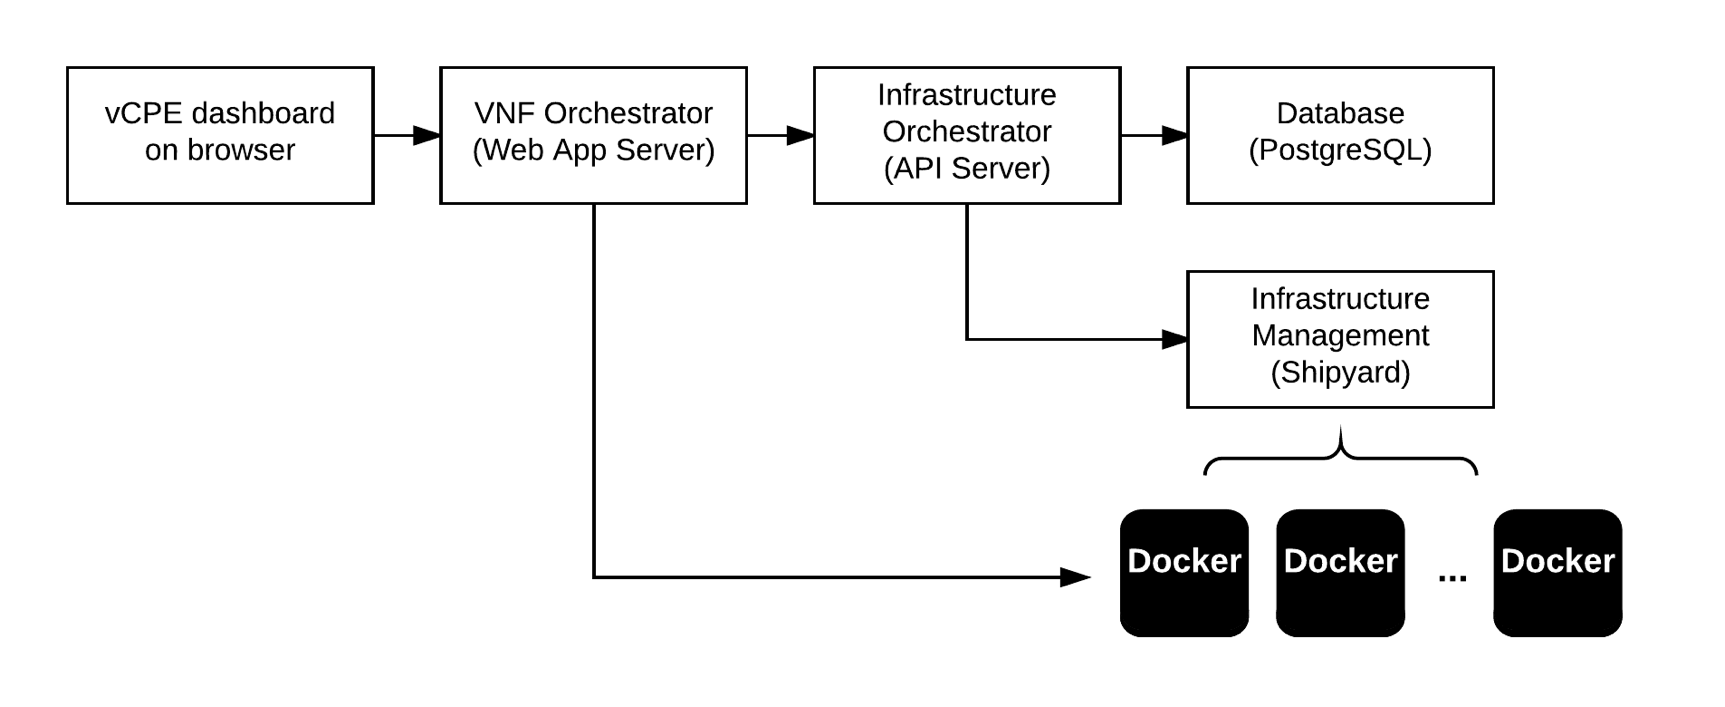
\includegraphics[width=3in]{./figures/desc_vcpe_framework}
\caption{Architecture of the vCPE framework.}
\label{fig:desc_vcpe_framework}
\end{figure}

\subsubsection{Infrastructure Controller}

The infrastructure controller comprises a Docker management server that can manage the Docker resources like containers and images and a OpenStack server that can manage the VM resources. The infrastructure controller does not manage customer authentication or maintaining the state of the running service; however, it follows the request from the infrastructure orchestrator to create, delete, start, stop, and inspect containers and VMs.

\subsubsection{Infrastructure Orchestrator}
The infrastructure orchestrator plays a key role in our system. It connects and automates the workflows when our services are deployed. When a customer subscribes to our service, the infrastructure orchestrator first authenticates the customer, calls the infrastructure controller to create a container or a VM for the customer, and then updates the information in the database. The infrastructure orchestrator controls the entire life-cycle of our vCPE services.

\subsubsection{Cloud Database}
The cloud database is used for restoring the meta data of our vCPE services, which include each customer’s credentials, customer’s container/VM settings, and virtual CPE service states. The cloud database employs PostgreSQL, which is an open source, easily customizable and object-relational database system. Only the infrastructure orchestrator has permissions to access the cloud database.

\subsubsection{VNF Controllers}
VNF controllers comprises an SDN controller developed using Ryu framework \cite{web:ryu} and a remote launcher module. The SDN controller does not have a remote launcher module for remotely executing an SDN controller. We built a light-weight server as a launcher module to resolve this problem. The remote launcher module monitors the SDN controller process ID (PID) and kills the SDN controller PID on demand. Once the infrastructure controller  creates the container or the VM, the remote module will initially runs, waiting for requests from VNF Orchestrator. The details of an SDN controller design are presented at Section \ref{sec:mft}.

\subsubsection{VNF Orchestrator}
The VNF orchestrator is a web application server hosted on Amazon web server, and provides to customers an online dashboard for vCPE services management and configuration. Through the web-based UI provided by the VNF orchestrator, customers can subscribe to the desired service without typing any command through the command line interface. After receiving the subscription message, the VNF orchestrator requests the infrastructure orchestrator to create a new VNF controller, and then sends the virtual CPE configuration to the new VNF controller. Based on configuration demands under different conditions, the network administrator can select any of the listed network functions on the dashboard, such as Firewall, NAT, DHCP, and quality of service (QoS) management.



\subsection{Network Functions}
The proposed vCPE service provides the following network functions.

\subsubsection{Firewall}
The firewall service can filter the packets based on packet header fields, including MAC address, IP, and layer4 protocols. The network manager can add new rules or remove rules from the access control list through our vCPE GUI.

\subsubsection{NAT}
The NAT service is a network function that can remap the IP address to another one. The source NAT (SNAT) is typically used by internal users (inside a private network) to access the Internet (outside the network). The network function uses the action set-field action, which is defined by OpenFlow protocol for rewriting packet header fields. Through the vCPE GUI interface, the network manager can set up the WAN port of the SDN switch, public IP, default gateway, and local network address when using this function.

\subsubsection{DHCP}
DHCP dynamically allocates IP addresses to hosts.
To implement this function, the SDN controller copes with UDP packets that use port 67 and 68.
The SDN controller generates DHCP Offer packets and DHCP Ack packets in reply to DHCP Discover packets and DHCP Request packets received from the hosts.

\subsubsection{Forwarding}
The forwarding Service is a basic service that forwards traffic to its destination. We used the Mac address learning concept to implement the forwarding function.

\subsubsection{QoS}
QoS is used to control the traffic flows of a network and prevent the traffic from exceeding the network capacity and leading to congestion. Therefore, we implemented bandwidth management using meters which are defined within OpenFlow protocol 1.3, to set the limitation on the bandwidth. In addition to achieving network functions virtualization with SDN technology, we enabled network administrator to manage and monitor a network more easily. Consequently, we can offer the user the highest network quality under limitations on network resources without traffic congestion.
In this study, we integrated QoS with a flow classification engine and offered two methods of bandwidth management:

\begin{itemize}[\IEEEsetlabelwidth{Z}]
\item set the limitation on the bandwidth of a specific host;
\item set the limitation on the bandwidth of a specific application.
\end{itemize}



\subsection{Application Identification}
Application identification entails identifying the application of each flow to enable QoS management system
to execute bandwidth control or distribution at application level \cite{dynamic-qos-umeida}, \cite{network-slicing-asia-pacific}. The application name indicates the name of the application which establishes the flow. A flow is defined by a 5-tuple (source IP address, source port, destination IP address, destination port, and transport layer protocol). Applications include desktop applications, native mobile applications, and web-based applications, such as Facebook, Skype, YouTube, Instagram, Line, and WeChat. We used supervised machine learning (ML) and a method based on the inspect of domain name service (DNS) responses for flow classification. After the application identification system classifies a flow under an application name, it sends the classification result to a server connected to a database. The server stores the classification result in the database, and waits for requests from the QoS management system. This process is described in detail in Section \ref{sec:app_identification}.




\section{Network Function With Multiple Flow Table Management Model} \label{sec:mft}

\begin{figure*}[!t]
\centering
\includegraphics[width=6in]{./figures/mft_table_overview}
\caption{Flow table order of vCPE service.}
\label{fig:mft_table_overview}
\end{figure*}

\subsection{Multiple Flow Tables Strategy}
In subsection \ref{ssec:desc_nfv_overview}, we introduce the vCPE service design architecture. The network functions are managed through cooperation between the SDN controller on the cloud and SDN switch at the local network gateway. The controller transforms the network functions into a series of OpenFlow rule requests and sends it to the SDN switch. Following the orders from the controller, the SDN switch inserts the rules into its flow tables, examines the incoming packets against the flow entry match fields, and executes the actions in matching rules. The flow table \cite{sdn-ft} defines all matching and corresponding processing, thus playing an important role in the executive network function.

We found that a single flow table restricts the implementation of our network functions. In \cite{onf-multi-tables}, two conditions under which a single flow table is too restrictive were reported. The first is a condition where a single packet must perform independent actions based on matching with different fields. The second is a condition where the packet requires two-stage processing. To satisfy both conditions, we implemented the network functions by using a multiple flow table strategy.

Before we discuss about the multiple flow table strategy, we introduce the pipeline of OpenFlow flow table first \cite{sp:openflow13}. The processing of each packet always starts at the first flow table. When processed by a flow table, the packet is matched the flow entries of the flow table and adds corresponding action to the instruction set. The packet can executes the instrcution set immediately, or execute after finishing the journey in switch. A flow entry can direct a packet to next table by go-to action. In our multiple flow table management model, we will set the go-to-next-table action as the table-miss action. Therefore, the packet is processed table-by-table in a certain sequence.

In a multiple flow table strategy, it is most important to determine which flow table the rules should be inserted into. We used the network function as a demarcation, that is, SDN applications responsible for specific network functions inserted rules into one specific flow table to enable us to focus on the design of the network function itself. However, the order of the flow table and the sequence of the network functions become crucial. This can be addressed by considering the type of match and action in the rules generated by the network function.

The network functions of vCPE services are the firewall service, NAT, DHCP, forwarding, and QoS. The order of each function was determined as shown in Fig. \ref{fig:mft_table_overview} (note that the flow tables are counted from zero). Each packet In the following sections, we introduce the method of implementing these network functions, the type of rules to be inserted into the SDN switch, and the effect of these rules on deciding the order of the flow tables



\subsection{Service Control}
Service control is used to enable or disable services. To enable a service, the table-miss rule should be modified. A packet-in rule is always placed in the flow table of the last active service as a table miss in case there is no corresponding rule. To enable the service chain, the rules of each service except the last service contain an additional action, ``go to next flow table'', which enables the packets to continue to pass through all active services.

To disable a service, we must not only modify the table-miss rule but also add an enforce rule. Each enforce rule has maximum priority with the action, ``go to next flow table''. It indicates that packets still pass through the disabled service’s table, but ignore other rules and proceed to the next flow table.



\subsection{Firewall}
The firewall service can dynamically block traffic and prevent the packets from causing a packet-in event.

On the dashboard, we can specify the blocking policies. There are 3 kinds of policies:
\begin{itemize}[\IEEEsetlabelwidth{Z}]
\item block any traffic from a source IP or destination IP address;
\item block traffic based on known layer 4 protocols, such as SSH and HTTP;
\item block traffic to customize layer 4 ports of a host.
\end{itemize}

For different policies, the controller applies corresponding rules to the SDN switch. After the policies are set, the blocking rules are immediately installed. Subsequently, any traffic that satisfies the blocking criteria is dropped. Normal traffic is unaffected.

As shown in Table \ref{table:fw}, all the actions of flow entries are dropped. The first rule illustrates that SSH connection with the source IP address 192.168.2.1 is blocked. The second rule indicates that the flow entry blocks the Telnet protocol.

In our multiple flow table model, the firewall service is located in flow table 1 because once packets are detected by the blocking rules, they do not need to be applied to any other services. The packets that satisfy the blocking rules are immediately dropped, and their journey in the flow table ends. The other unblocked packets pass all blocking rules and finally satisfy the table-miss rule, which allows the packets to proceed to the next flow table. The action of the firewall is different from those of other services, because in other services, irrespective of the actions taken with the packets, the packets must proceed to the next flow table.

% firewall example table
\begin{table*}[!t]
\caption{Firewall rules in Flow Entry}
\label{table:fw}
\centering
\begin{threeparttable}
\begin{tabular}{|l|l|l|l|l|l|}
\hline
IP proto & IP src      & IP dst       & L4 sport & L4 dport & action \\ \hline
TCP      & 192.168.2.1 & *            & *        & 22       & drop   \\ \hline
TCP      & *           & *            & *        & 23       & drop   \\ \hline
\end{tabular}
  \begin{tablenotes}
    \item[] Symbol * represents wildcard (matches any value).
  \end{tablenotes}
\end{threeparttable}
\end{table*}



\subsection{NAT}
The NAT service allows numerous hosts to use one public IP address for connecting to the network. To achieve this, the SDN controller must set the packet header field. Because the SDN switch sets the field, the first packet must proceed to the controller. When the controller adds the flow to the SDN switch, the packet does not proceed to the controller. This can reduce the burden on the controller.

Following is an example that illustrates the modification of the IP address and port number by using the NAT service. For an outgoing packet, the SDN switch does not have any flow entry in the flow table, and hence, a packet-in event is triggered initially. The packet that is sent by a private network host is sent to the SDN controller, and the packet header fields are modified using the set-field action. The source IP address and source port number of the outgoing packet are modified to a public IP address and a new port number is remapped for NAT. For the incoming packet, the destination IP address and destination port number are modified to fit the private IP address and port number. Subsequently, the SDN controller adds these flow entries to the SDN switch; all packets must be sent to the controller

In Fig. \ref{fig:mft_nat}, the public IP address of NAT is 140.114.71.178, and the host private IP address is 192.168.8.254 with the port number 7878. The client sent the packet to a server with the IP address 140.114.71.177 and port number 9898.

As shown in Table \ref{table:nat}, when the host sends the packet to the server (outgoing), a packet-in event is triggered, and the packet is sent to the controller. The set-field action modifies the source IP address to a public IP address of NAT, 140.114.71.178, and the source port to 2000. When the server sends the packet back to the client (incoming), the packet header field is modified. The destination IP address and destination port number are modified to 192.168.8.254 and 7788, respectively.

In the single flow table framework, two rules must be added to the SDN switch to match the outgoing and incoming situations. First, we predicted that the NAT service must be placed in the last table of the multiple flow table framework because the NAT service must set the packet header fields and enable connection to the outside network. Most importantly, the SDN switch is placed according to the order of tables to match the field. The outgoing and incoming situations must be considered. In consideration of all the aforementioned factors, we place the NAT service in the first and last tables in our multiple flow table framework.

\begin{figure}[!t]
\centering
\includegraphics[width=3in]{./figures/mft_nat}
\caption{Example of modification of IP address and port number by NAT service.}
\label{fig:mft_nat}
\end{figure}

% NAT example table
\begin{table*}[!t]
\caption{Flow entry for modifying the packet header fields}
\label{table:nat}
\centering
\begin{tabular}{|l|l|l|l|l|l|}
\hline
            &IP src          & IP dst          & L4 src port  & L4 dst port & action                                                                            \\ \hline
1. outgoing &192.168.8.254   &140.114.71.177   & 7878         & 9898        & \begin{tabular}[c]{@{}l@{}}IP src $\,\to\,$ 140.114.71.178; \\ L4 src port $\,\to\,$ 2000\end{tabular} \\ \hline
2. ingoing  &140.114.71.177  &140.114.71.178   & 9898         & 2000        & \begin{tabular}[c]{@{}l@{}}IP dst $\,\to\,$ 192.168.8.254; \\ L4 dst port $\,\to\,$ 7878\end{tabular} \\ \hline
\end{tabular}
\end{table*}



\subsection{DHCP}
The DHCP service implements the DHCP protocol to dynamically assign IP addresses to hosts. A DHCP operation uses the UDP protocol. Clients use port 68 as the source port and port 67 as the destination port. By contrast, the server uses port 67 as the source port and port 68 as the destination port. Our system can handle packets to realize the DHCP service.

This service is executed through the following steps:
\begin{enumerate}
\item The controller adds a DHCP rule for DHCP packets when the service is enabled.
\item All packets match this DHCP rule, causing a packet-in event.
\item The controller determines whether a packet is a DHCP discovery packet. If so, the controller assigns an IP address, generates a DHCP offer, and then performs a packet-out event. If not, the controller determines whether it is a DHCP request. If the result is positive, the controller generates a DHCP acknowledgement and then performs a packet-out event.
\end{enumerate}

Our system supports multiple flow tables; however, a specific flow table for the DHCP service is not required because only one rule is installed for all hosts who request the DHCP service. When the service is disabled, the DHCP rule is deleted, and the packets continue to pass through our service chain. The subsequent DHCP packets can reach other DHCP servers by forwarding service.



\subsection{Forwarding} \label{ssec:forwarding}
In the forwarding service, when the first packet in a new connection is incoming, a packet-in event occurs because no corresponding rule is present. When the controller receives the packet, it records the IP-layer information, including the source IP address, destination IP address, input port number, source MAC address, and destination MAC address. By using the recorded information, the controller can install a 5-tuple forwarding rule with out-port action for this connection, and the subsequent packets do not need to undergo the packet-in event. The 5-tuple comprises the source IP address, destination IP address, network layer protocol, source layer 4 port, and destination layer 4 port.

To gather per-session statistical information, 5-tuple rules are required. Therefore, rules based on the MAC address are not added. The controller installs a pair of dummy rules for every connection, and then requests the switch to obtain current flow statistics every second. Thus, the real-time bandwidth statistics of each connection can be obtained by merely subtracting the byte count from the byte count of the last second.



\subsection{QoS}
QoS is mainly used for traffic control. Two management functions are provided for QoS. We first introduce three strategies and then discuss the flow table order of QoS in the multiple table model.

\subsubsection{Rate Limitation of Hosts}
When some hosts utilize a high network bandwidth, the speed for other hosts slows or traffic congestion occurs. To prevent these effects, rate limiting is used to control the rate of traffic from a host. For implementing the host rate limitation, we first create a meter for the desired bandwidth and then add a flow, of which the match is the host’s MAC address and the action is the meter.

This method is illustrated in \ref{fig:mft_qos_rate_host}. In T0, host 1 and host 2 are not limited yet. Because host 2 utilizes a substantial amount of bandwidth from the network in T0–T1  the network administrator sets the host 2 rate limit to 400 Kbps. When the controller receives this request, marked as (a), it creates a meter with meter id = 1 and bandwidth = 400 Kbps and sets the rule in the flow table with the destination MAC address = MAC address of Host 1 and meter = 1. According to our new flow table, it limits the rate of the target host. Then, the traffic from Host 2 is reduced and immediately limited to 400 Kbps. A similar situation occurs for Host 1 in T2. The administrator chooses to set Host 1 under 600 Kbps, marked as (b), and then the traffic from Host 1 is limited to 600 Kbps.

\begin{figure}[!t]
\centering
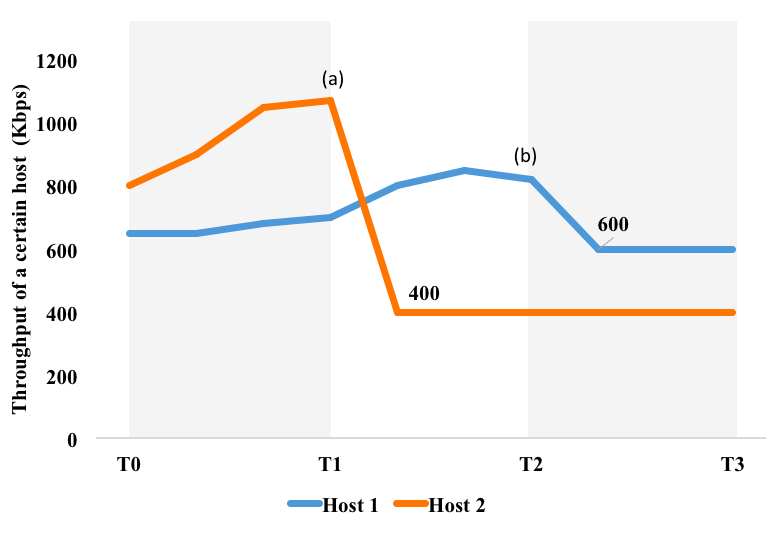
\includegraphics[width=3in]{./figures/mft_qos_rate_host}
\caption{Illustration of rate limiting for a certain host}
\label{fig:mft_qos_rate_host}
\end{figure}

\subsubsection{Rate Limitation of Applications}

An increasing number of network applications such as online games, video streaming, and conference calls are used. Therefore, substantial traffic exists in the network. Consequently, we integrated a flow classification engine to identify which application the flow belongs to. The integration scenario is presented in Fig. \ref{fig:class_classifying}.

To rate the limit for a certain application, we must first gather per-flow statistical information. When a connection is created, the first packet of the connection is handled by the forwarding service and the 5-tuple rules are added into the SDN switch to obtain the bandwidth information of the per-flow connection (see Section \ref{ssec:forwarding} for details). With the classified result of application identification, the application type of each connection can be determined.

When the network administrator requests to rate limit a certain application to a certain bandwidth, the bandwidth is equally distributed to each connection of the application. The controller sets all flows that belong to the same application into the same meter, and the bandwidth of the meter is modified to achieve the desired value. For example, suppose that we can determine which flows belong to an application through the flow classification engine. This application is to be limited to 1000 Kbps. In T0 (Fig. \ref{fig:mft_qos_rate_app}), three connections belong to this application, and the bandwidth of the meter to each link is set as 333 (1000/3) Kbps. In T2, two connections are added to this application, and the bandwidth of the meter to each link is reset as 200 (1000/5) Kbps. In T2, one connection is obtained in this application, and hence, the bandwidth of the meter to each link is reset as 250 (1000/4) Kbps. However, the sum of bandwidth from this application should always be 1000 Kbps. In other words, the bandwidth is dynamically adjusted.

It is worth noting that we did not change any rules in flow table; we merely change the bandwidth of the correspond meter in the meter table to reduce the overhead of switch and controller.

\begin{figure}[!t]
\centering
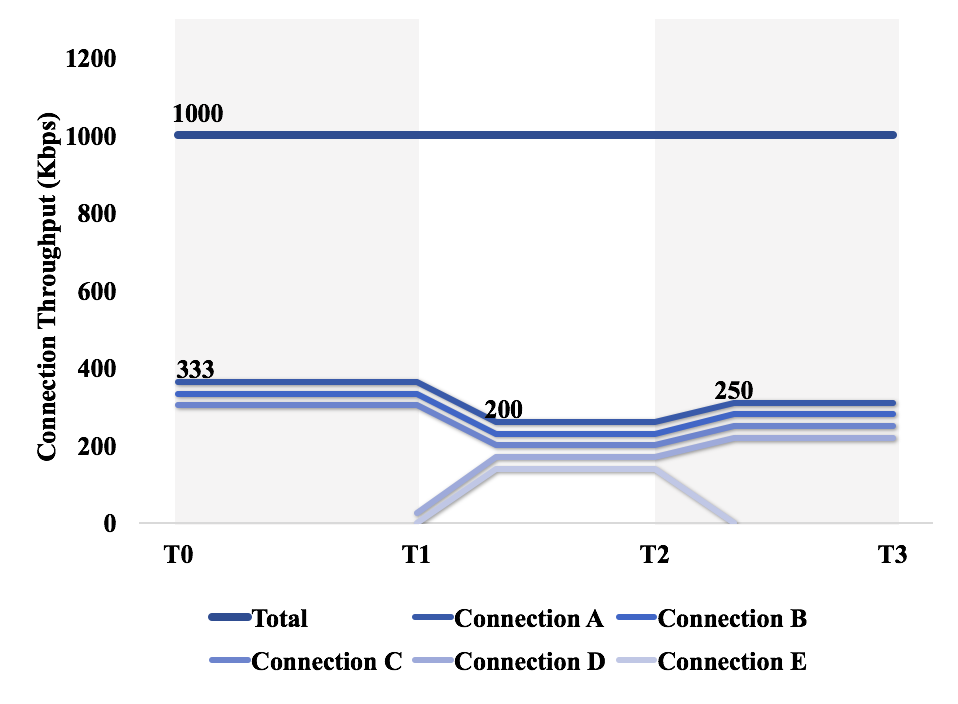
\includegraphics[width=3in]{./figures/mft_qos_rate_app}
\caption{Illustration of rate limiting for a certain application.}
\label{fig:mft_qos_rate_app}
\end{figure}

\subsubsection{The Flow Table Order of Forwarding and QoS Service}
Because the location of NAT, DHCP, and the firewall have been determined, we only need to decide the arrangement of QoS and forwarding. Assume that we place the QoS flow table after the forwarding flow table. In addition, we have only two services enabled, forwarding and QoS; therefore, the packet-in rule is in the last flow table of active service, Qos service. Then, suppose that a host is not limited by QoS policies. The first packet is not affected in both arrangements. For the subsequent packets, a difference can be observed. The packets that satisfy the rules in the forwarding flow table can not match rate limit rules in QoS flow table, because the host is not limited by QoS service; instead. As a result, the packets cause packet-in events by matching the packet-in rule in QoS service. This is unexpected because the packets already get the out-port action from the forwarding service. That is, it is not necessary to send these packet go to controller, and any packet-in event increases the controller’s load.

To reduce this load on the controller, we place the QoS flow table ahead of the forwarding flow table. In this scenario, all packets that pass through the QoS flow table continue to proceed to the forwarding flow table without satisfying any QoS rules. Then, all packets except the first packet are merely forwarded by the forwarding service instead of causing packet-in events. Thus, the controller’s load decreases.



\section{Application Identification Method}\label{sec:app_identification}
To enable the QoS management system to control or distribute bandwidth at the application level, we designed and implemented an application identification system (also called flow classification system) to identify the application that establishes each flow. In other words, the application identification system can classify each flow under an application name in real time, rather than a rough category or a transport layer protocol. The corresponding application name of a flow indicates the name of the application that establishes the flow. We use supervised ML and a method based on the inspection of DNS responses for flow classification. The system analyzes the packets with the transport protocols TCP or UDP. Except for DNS responses, the system reads only headers to obtain the transport layer information of packets without inspecting their payload



\subsection{Architecture of Application Identification System}
The application identification system comprises a training phase (also called the preparation phase) and a classification phase; their architectures are presented in Figs. \ref{fig:class_training} and \ref{fig:class_classifying}, respectively. These architectures can be integrated to perform training and classification simultaneously.

\begin{figure}[!t]
\centering
\includegraphics[width=3in]{./figures/classification_training}
\caption{Architecture of our application identification system in training phase.}
\label{fig:class_training}
\end{figure}

\begin{figure}[!t]
\centering
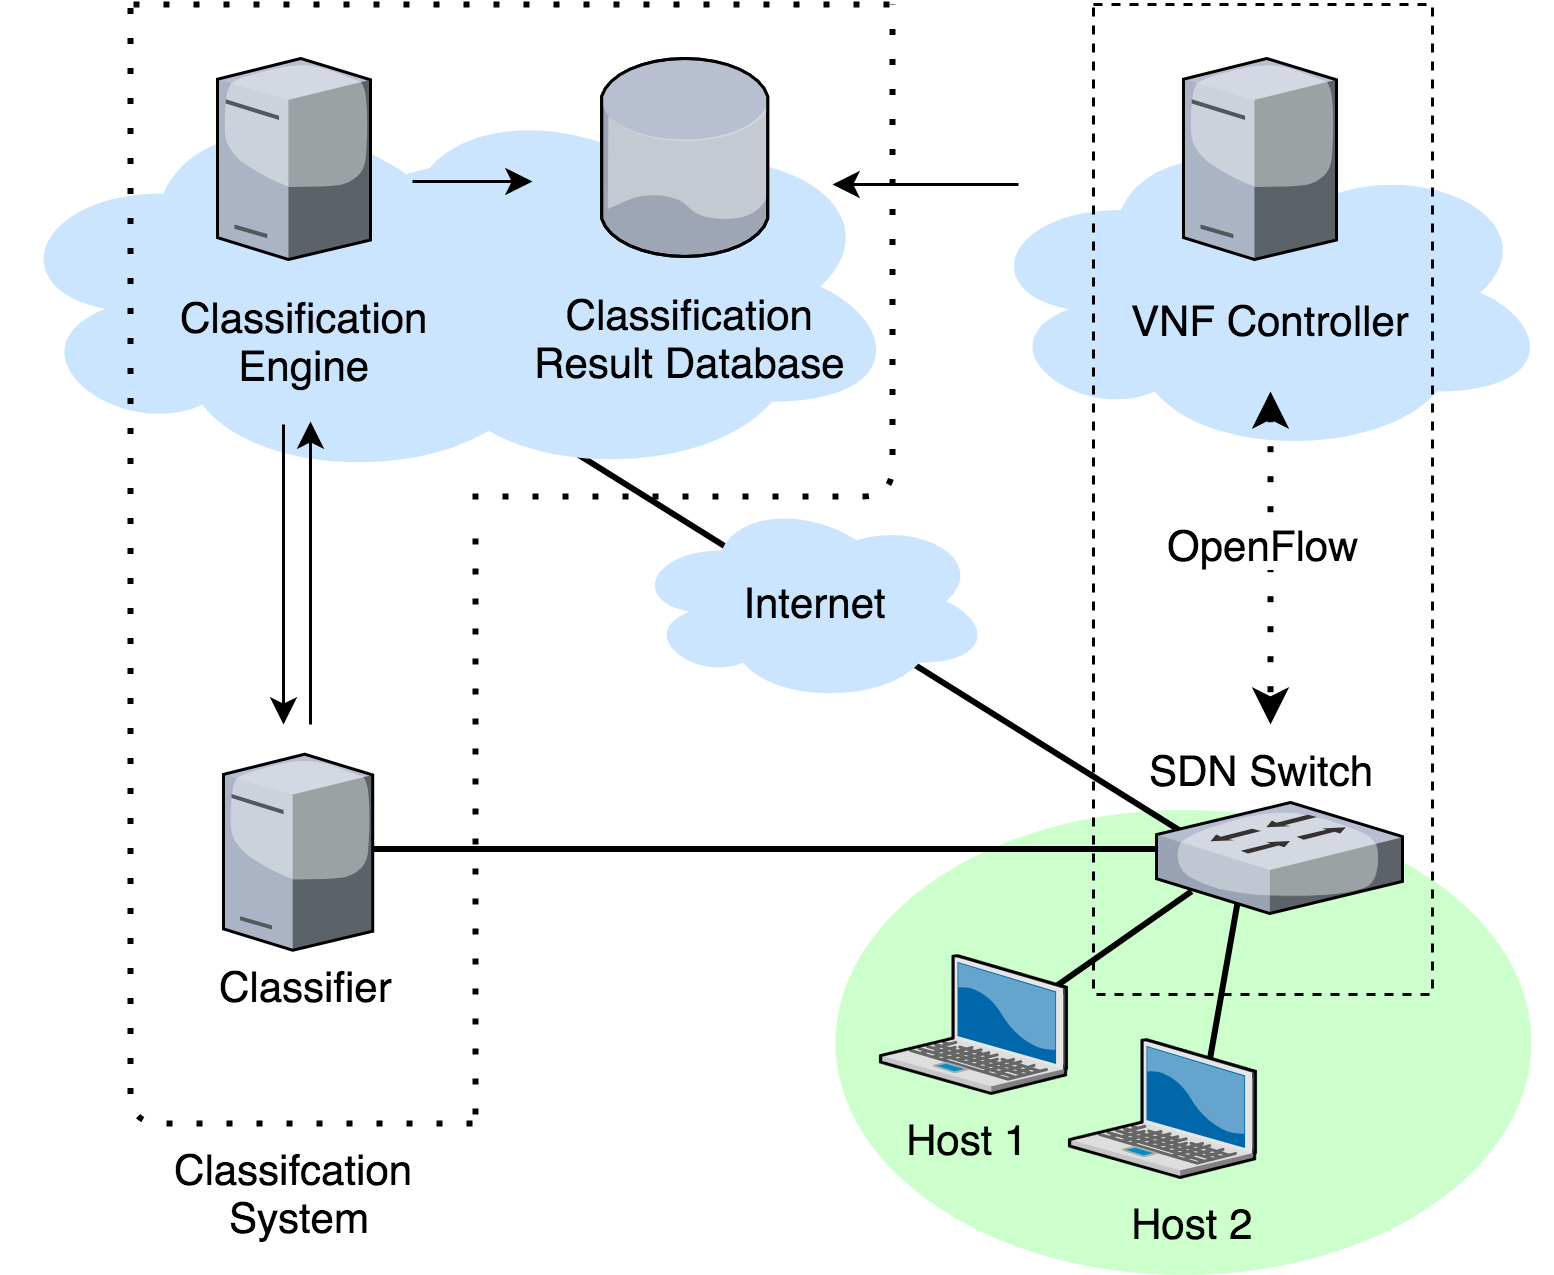
\includegraphics[width=3in]{./figures/classification_classifying}
\caption{Architecture of our application identification system in classification phase.}
\label{fig:class_classifying}
\end{figure}



\subsection{Overall Procedure of Application Identification}
In the training phase, we generate data required for the proposed method. In the classification phase, if a flow meets some requirement, we use the method based on the inspection of DNS responses for classification; otherwise, we use supervised ML.



\subsection{Procedure of Supervised ML}
The architecture in the training phase is presented in Fig. \ref{fig:class_training}. The flow classification engine is used for building a classification model by using training data from the trainer. The model is updated when new training data are received. The trainer is used for analyzing traffic from the mirror port to obtain flow attributes. After the trainer calculates the attributes of a flow, it obtains the ground truth of the flow from the scanner or app meta server to generate training data and sends the training data to the flow classification engine. The app meta server is used to store mappings of the 5-tuple and ground truth from the scanner and accept queries from the trainer. The scanner is used to obtain mappings of the 5-tuple and ground truth from the OS. The architecture in the classification phase is presented in Fig. \ref{fig:class_classifying}. In this architecture, the flow classification engine uses flow attributes from the classifier and classification model to obtain a classification result and sends the classification result to the classifier. The classifier analyzes the traffic from the mirror port to obtain flow attributes. After the classifier calculates the attributes of a flow, it uses them to order the classification result from the flow classification engine if required.



\subsection{Definition of Ground Truth of Flow in Supervised ML}
Ground truth of a flow can be defined based on server (owner of server, category of service, or name of application providing service in server), client (category or name of application in client, or name of executable file in client), or communication (transport layer protocol, or application layer protocol). Similar with\cite{Qazi2013} \cite{Iwai2016}, we define ground truth of a flow based on the application establishing the flow in client for desktop applications and native mobile applications. As for web-based applications, we define ground truth of a flow based on domain name of web service.



\subsection{Method to Obtain Ground Truth of Flow in Supervised ML}
We install our software on various devices establishing the flows. We call the software scanner. Scanner has different implementation versions for different operating systems (OSs). For desktop applications on Windows, trainer acts as scanner. It uses Windows API and local port of the flow to obtain the ground truth of the flow. As for Mac OS X, scanner calls the UNIX command ``lsof'' and parses the result to obtain lists of 5-tuples, process IDs (PIDs), and application names. Then scanner uses the PID and ``ps'' to obtain corresponding complete application names. As for native mobile applications on iOS, scanner uses a method similar to that used on OS X. However, we have to install package of UNIX command and jailbreak the iPhones before scanner runs.  As for native mobile applications on Android, scanner calls ``cat /proc/net/tcp'', ``cat /proc/net/tcp6'', and ``cat /proc/net/udp'', and parses the results to obtain mappings of 5-tuples and UIDs. Next, the Android API and UIDs are used to obtain corresponding application names as ground truth. Finally, mappings of 5-tuples and application names are obtained. For iOS and Android, scanner has to run in background.

As for web-based applications, we implemented a browser in Java. We let it run in Windows. It has two main modules. One browses websites to generate traffic. It browses only one website at a time. The other module obtains the PID of the browser module, shortens the domain name of the currently browsed website to act as the application name, and receives requests from Scanner. When scanner in Windows detects an active flow, it uses the Windows API to check what process established the flow. It obtains the process name and the PID of the process. When it encounters a process name that is ``java.exe'' or ``javaw.exe'', it sends the PID to the browser. If the PID is the browser’s PID, the browser sends the application name to Scanner to act as the ground truth of that flow.

\subsection{Flow Attributes Adopted in Supervised ML}
In ML, when the system calculates flow attributes, we use only the transport layer information of packets with a payload. Moreover, we use the application round (APPR) proposed in \cite{classfication-cloud} to analyze the flow behavior. We use the number of packets, packet size, transmission time, transmission direction, throughput, and APPR to define flow attributes, such as total number of packets transmitted by the client, size of data transmitted by the server in Round N, and the average transmission time of each packet in Round N.A total of 69 attributes are defined, as reported in our previous study \cite{Chia-Chin-master}.



\subsection{Procedure of Calculating Flow Attributes}
When each packet comes in, the system creates or updates the information of the flow of the packet. The system stores the information of each flow simultaneously. When a flow meet the requirement to be summarized to produce statistical flow attributes, it takes less than 0.1 seconds to summarize that flow. The attributes of most flows, in our experience, require less than 10 seconds to calculate. After system calculates flow attributes, it takes less than 0.1 second to classify the answer.



\subsection{Algorithms Adopted in Supervised ML}
We use algorithms implemented by Weka, an open-source ML tool developed at the University of Waikato. We call the Weka Java API to build the classification model. We did model selection on all algorithms provided by Weka 3.8.0. To reduce effort, we generated two small data sets containing approximately 100 applications to act as a training data set and a classifying data set; this was done to avoid 10-fold cross validation on a testing data set. These data sets can be used for model selection, but they were not the data sets that were used to verify accuracy in the experiment of this study. Finally, considering accuracy, time to build classification model, memory usage to build and apply classification model, we use three algorithms, RandomSupSpace with RandomTree [35], FilterClassifier with discretization and RandomTree, and RandomCommittee with RandomTree. For a flow, we derive the classification result of each algorithm, and do majority voting to obtain final classification result.

We studied the detail of these algorithms, and posited two reasons why these algorithms achieve high accuracy. One is that all of them are based on the random tree pattern, a type of decision tree that reduces overfitting by randomly selecting a subset of attributes, then selecting one attribute to split the node. The second reason is that two of them perform ensemble learning, a type of learning that is favorable for reducing overfitting to enhance accuracy.



\subsection{Procedure of the Method Based on Inspecting of DNS Responses}
Similar with \cite{Plonka_flexibletraffic}, we do flow classification based on DNS responses. However, different from\cite{Plonka_flexibletraffic}, we link IP addresses in DNS responses to application names derived from OS of client, and use the IP addresses which have been linked to only one application to classify.

More specifically, in the training phase, we collect the mappings of the server IP address and application name. A mapping of the server IP address and application name indicates whether the application has ever established a connection with the server, the IP address of which is identified as the server IP address, and the server IP address has ever occurred in any DNS response captured. In the classification phase, we do not use server IP addresses with more than two corresponding applications among the mappings for classification. We use only those server IP addresses with one corresponding application in the mappings for classification. When the system detects a flow, we examine whether the source IP or destination IP address of the flow matches any of the server IP addresses. If it matches, we consider the corresponding application name as the classification result; otherwise, we use flow attributes of the flow and the classification model of supervised ML for classification.





\section{Performance Evaluation}
\subsection{Multiple Table Performance}

\begin{figure}[!t]
\centering
\includegraphics[width=3in]{./figures/evaluation_nat_scenario}
\caption{Multiple Table Performance Evaluation Scenario}
\label{fig:evaluation_nat_scenario}
\end{figure}

\begin{figure}[!t]
\centering
\includegraphics[width=3in]{./figures/evaluation_nat_result}
\caption{Results of Multiple Table Performance Evaluation}
\label{fig:evaluation_nat_result}
\end{figure}

Implementing a single flow table framework is easier than implementing a multiple flow table framework; however, multiple flow table frameworks are more flexible. To verify the efficiency of the multiple flow table vCPE framework, we conducted an experiment by using the NAT service to compare the throughput between single flow table vCPE and multiple flow table vCPE.

An overview of the experimental environment is presented in Fig. \ref{fig:evaluation_nat_scenario}. The NFV controller was run on the Dell PowerEdge R630 rack server, and the Pica8 P-3290 switch \cite{pica8-switch} was used as the SDN switch. We used iPerf2 \cite{iperf} to generate network traffic. The iPerf server connected the public IP address with 140.114.71.178, and then the iPerf client connected to the SDN switch and was controlled by the NFV controller. The NFV controller ran the NAT service, but used different frameworks, a single flow table and multiple flow table.

We used iPerf to generate UDP packets and send them to the server from the client, and we fixed the bandwidth at 100 Mbps. In this experiment, different payload sizes were used to evaluate the performance of the flow tables. As shown in Fig. \ref{fig:evaluation_nat_result}, the throughput values indicate that the performance for large packets such as 1024 bytes and 1470 bytes was higher than that for small packets.

Because the NAT service is required to set the packet header field and a small payload tends to result in more packets being sent to the server simultaneously, the performance for larger packets is high. The throughput value of the multiple table framework is close to that of the single table framework. Thus, the multiple table framework is more flexible than the single table framework; however, the performance of the frameworks is similar (Fig. \ref{fig:evaluation_nat_result}).



\subsection{Accuracy of Application Identification}
\subsubsection{Testing Data Set}
1)	Testing Data Set: The testing data set comprised mappings of flow attributes and the ground truth. These mappings are also called rules. The testing data set was generated using our system in our lab in National Tsing Hua University in Taiwan. We manually operated applications to generate traffic. An application was used for approximately 50 min for each platform. The application identification system generated the rules and these rules were exported into a file for performing a ten-fold cross validation of the testing data set. A total of 14 659 rules were generated, and 137 applications were used if each platform version of an application is counted as one application. The testing data set did not contain all platform versions of each application that is in

\subsubsection{Validation Method}
Although the system can perform online training and classification, we performed offline training and classification, as shown in Fig. \ref{fig:evaluation_classification}. More specifically, we performed online training to analyze traffic, obtain the ground truth, and export the rules into a file. We then performed a tenfold cross validation of the rules. The ten-fold cross validation comprised ten rounds. We split the data set into ten subsets. At each round, we used one of ten subsets as the classification data set and the combination of the other subsets as the training data set. Then, we performed ten rounds, and each subset acted as the classification data set once. We implemented Classifier Light and Trainer Light, which acted as the classifier and trainer, respectively, without the function of analyzing traffic. Because the classification data set contained labels, we could calculate accuracy.

\begin{figure}[!t]
\centering
\includegraphics[width=3in]{./figures/evaluation_classification}
\caption{Evaluation of Application Identification.}
\label{fig:evaluation_classification}
\end{figure}

\subsubsection{Mapping of Category Names}
Mapping of Category Names: At each round of the tenfold cross validation, we applied name mapping to the training data set before we used it to build the classification model and we applied name mapping to the classification data set before we used it to calculate accuracy. The main reason for performing name mapping is that some applications have different ground truths in different operating systems. After name mapping, the testing data set contained 99 categories.

\subsubsection{Accuracy Matrices and Results}
Accuracy Matrices and Results: To evaluate the accuracy, we used precision, recall, and the F-measure (also called the F1 score), as shown in \ref{eqn_1}, \ref{eqn_2}, and \ref{eqn_3} \cite{muc4}. In each round of the tenfold cross validation, we calculated the precision and recall of each category to calculate the F1 score of each category. After ten rounds, we calculated the average F1 scores of each category in ten rounds. Table I presents the F1 scores in each category of the top 40 most popular applications in the testing data set. Next, we calculated the average F1 score of all categories in the ten rounds as 0.9062. The results (Table \ref{table:classification_result}) revealed that our system achieved high accuracy even there were up to 137 applications in testing data set, enabling QoS to effectively do bandwidth control or distribution at the application level in an enterprise network. Some applications achieved higher F1 score; we believe this happened because these applications had sufficient training data, simple flow combinations, or rarely query servers that accepted requests from numerous applications. We will gather more data to prove our belief, and add more applications to testing data set in the future.

\begin{equation}
\label{eqn_1}
Precision = \dfrac{True\ positive}{True\ positive\ +\ False\ positive}
\end{equation}

\begin{equation}
\label{eqn_2}
Recall = \dfrac{True\ positive}{True\ positive\ +\ False\ negative}
\end{equation}

\begin{equation}
\label{eqn_3}
F1\ score = \dfrac{2\times Precision\times Recall}{Precision + Recall}
\end{equation}

\begin{table}[!t]
\caption{AVERAGE F1 SCORE IN TEN ROUNDS of 40 POPULAR APPLICATIONS}
\label{table:classification_result}
\centering
\begin{tabular}{|l|l|l|l|}
\hline
\begin{tabular}[c]{@{}l@{}} Application \\ name\end{tabular}    & \begin{tabular}[c]{@{}l@{}}Average \\ F1 score\end{tabular}    & \begin{tabular}[c]{@{}l@{}}Application \\ name\end{tabular}  & \begin{tabular}[c]{@{}l@{}}Average \\ F1 score\end{tabular}   \\ \hline
OneDrive            & 0.991255            & Trello            & 0.988889           \\ \hline
gamerAnimad         & 0.985714            & Dropbox           & 0.985714           \\ \hline
AmazonMusi          & 0.977461            & MEGAsync          & 0.968889           \\ \hline
MEGAsync            & 0.968889            & BattleNet         & 0.967812           \\ \hline
Udacity             & 0.966667            & Lity              & 0.966427           \\ \hline
Tumblr              & 0.964624            & Asana             & 0.963492           \\ \hline
Skype               & 0.963117            & Twitch            & 0.963117           \\ \hline
TeamViewer          & 0.946667            & FileZilla         & 0.946429           \\ \hline
Agoda               & 0.944764            & TripAdvisor       & 0.942075           \\ \hline
Pinterest           & 0.936026            & BBCNews           & 0.931049           \\ \hline
LINE                & 0.923904            & Slack             & 0.920985           \\ \hline
Twitter             & 0.917906            & Youku             & 0.913925           \\ \hline
Evernote            & 0.912381            & Snapchat          & 0.912221           \\ \hline
Weibo               & 0.910872            & WeChat            & 0.906349           \\ \hline
GoogleDrive         & 0.896612            & Trivago           & 0.895406           \\ \hline
iTunes              & 0.890464            & Netflix           & 0.876234           \\ \hline
Facebook            & 0.868641            & Telegram          & 0.862222           \\ \hline
Airbnb              & 0.857029            & Spotify           & 0.856971           \\ \hline
Instagram           & 0.833465            & TED               & 0.829277           \\ \hline
Tmall               & 0.799747            & YouTube           & 0.713084           \\ \hline
\end{tabular}
\end{table}

\subsubsection{Performance Analysis}
In each round of 10-fold cross validation, after the flow classification engine received a training data set that had approximately 13241 rules, it spent around 6 minutes building a classification model on a workstation with ordinary hardware, including an Intel® Core™ i5-5200U CPU @ 2.20 GHz with 16 GB of RAM. When we only used supervised ML without our proposed method based on DNS responses, ClassifierLight read the classifying data set and asked the flow classification engine for a classification result. The system had approximately 1418 rules, and required around 5 minutes to verify accuracy. No out of memory errors occurred for the flow classification engine both in building classification models and classifying flows. We think this absence of errors happened because we chose a favorable classification algorithm so that memory usage was frugal and time required to build a model was short, even though the hardware was ordinary; 13241 rules and 99 categories existed in the training data set after name mapping.


\subsection{Evaluation of QoS When Host Bandwidth Is Limited}

We verify our function by downloading a file, because downloading is a situation that always consumes network resources in practice. We downloaded an image of Ubuntu 14.04 that was approximately 1 GB in size.


The NFV controller ran on the Dell PowerEdge R630 rack server and executed QoS (Fig. \ref{fig:class_classifying}). The Edge-Core AS5712-54X \cite{edge-core-switch} switch was used as the OpenFlow-enabled switch with the PicOS TM r2.6 operating system.

We used a desktop computer as the experimental host to record the bandwidth every 2 s. As shown in Fig 13, we started downloading the file without rate limiting; the rate was between 190 000 and 410 000 Kbps initially. At the \nth{10} second, we limited the host bandwidth to 1024 Kbps and added the rule matching the destination MAC address with a meter of 1024 Kbps. Then, we determined that the bandwidth from this host decreased and was limited to approximately 1024 Kbps immediately.

At the \nth{36} second, we canceled the limit to this host. In other words, we removed the meter field from the rule in the flow table. We observed that the bandwidth of the download from this host rapidly increased without rate limiting.

\begin{figure}[!t]
\centering
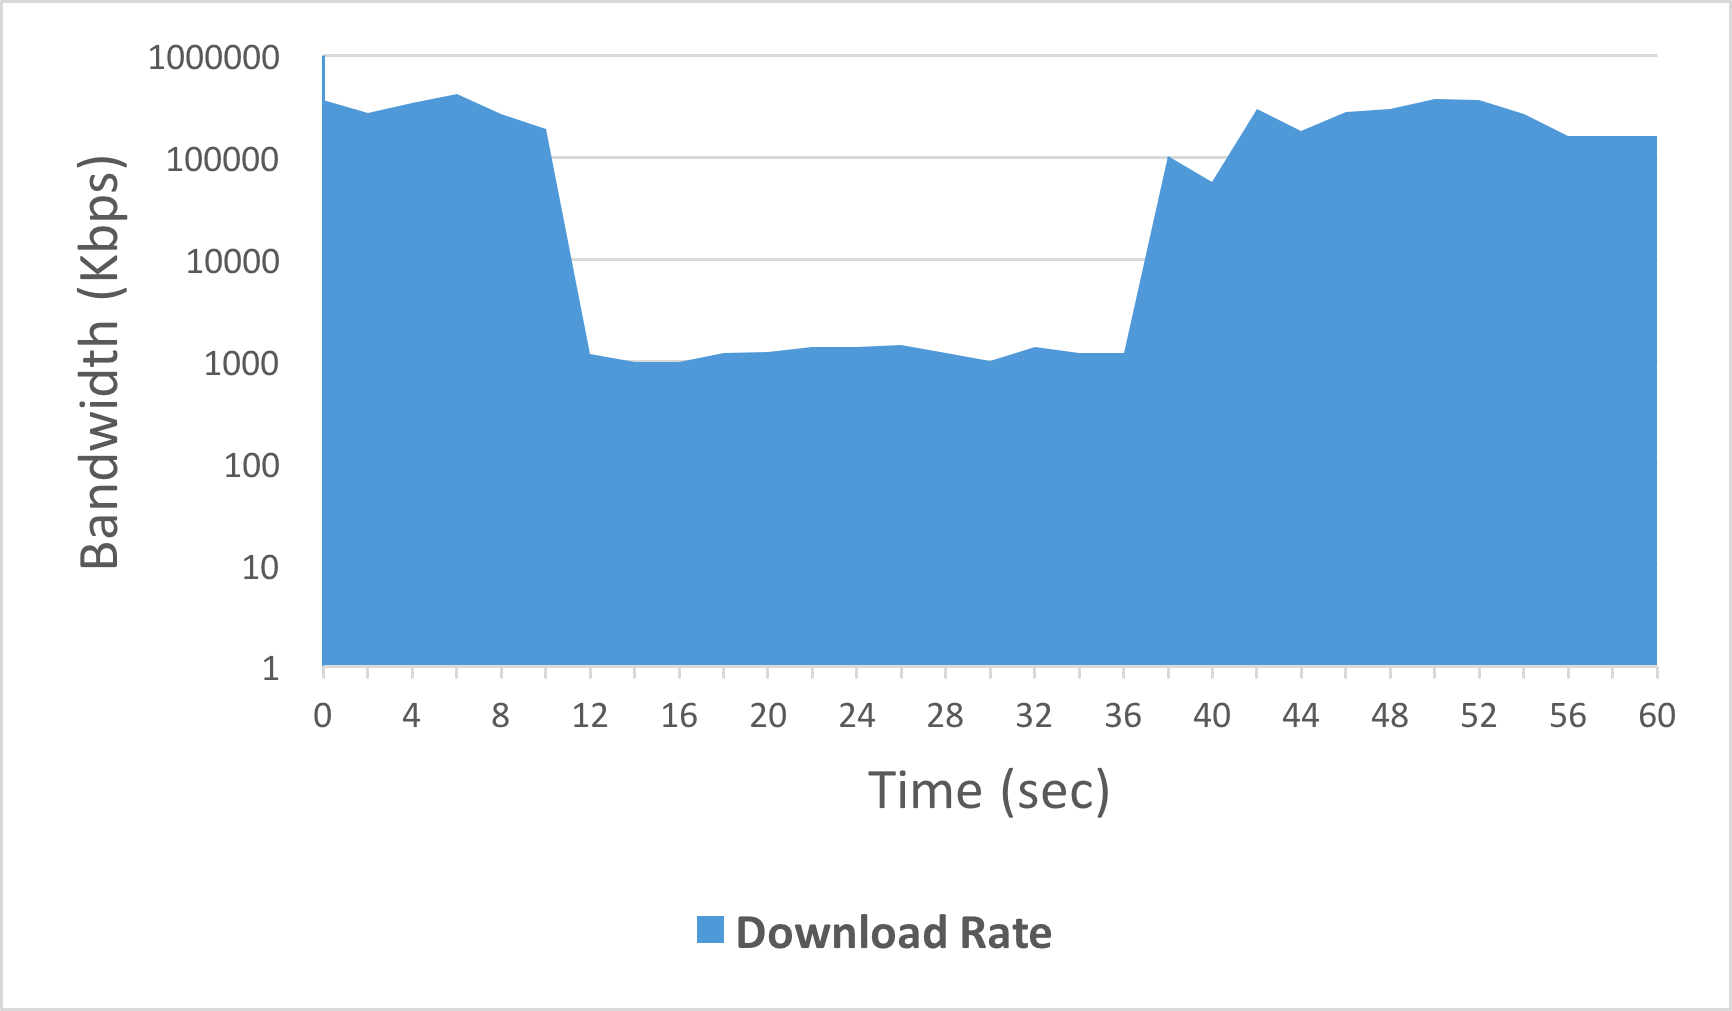
\includegraphics[width=3in]{./figures/qos_limit_host}
\caption{Limiting the download rate of a host.}
\label{fig:qos_limit_host}
\end{figure}

\begin{figure}[!t]
\centering
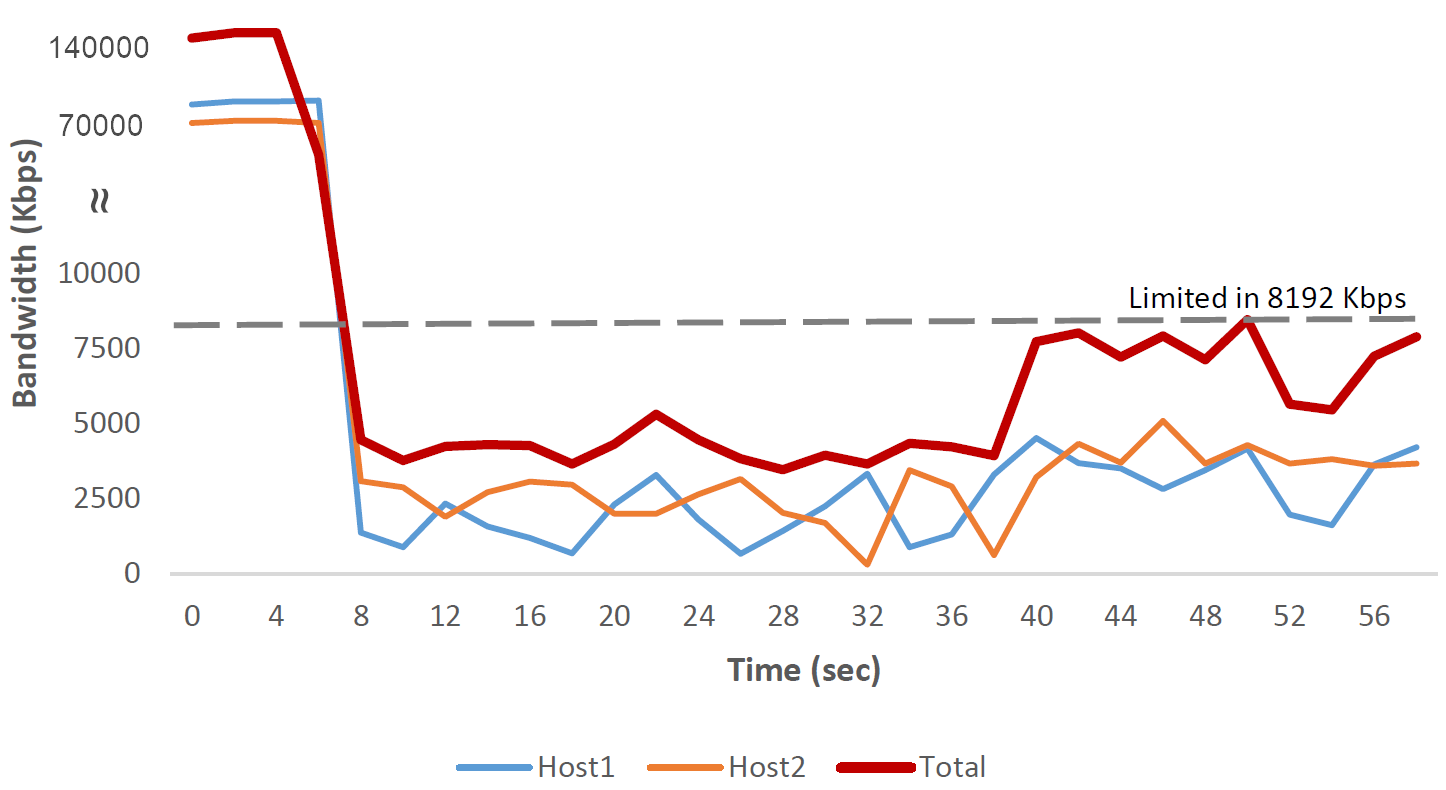
\includegraphics[width=3in]{./figures/mft_qos_rate_domain_app}
\caption{Limit the rate of Youtube in a network domain.}
\label{fig:mft_qos_rate_domain_app}
\end{figure}

\subsection{Evaluation of QoS When Application Bandwidth Is Limited}
Currently, numerous people use streaming applications, which consume a high amount of network resources. We employed application identification to determine the application to which each flow belongs.

In our experimental environment (Fig. \ref{fig:class_classifying}), we used a mirror switch to replicate all traffic from the SDN switch and to enable the application identification system to classify the flows according to the applications they belong to. The application identification system uploaded the identification results to the database.


Subsequently, the controller received the results from the database and updated the flow information of the applications. Therefore, we could use the flow information (5-tuple and identification results) to limit the application bandwidth.

We selected YouTube to verify our function for limiting applications and used three hosts (Host 1, Host 2, and Host 3) in the same network domain. Then, we limited the bandwidth of YouTube in this network domain (i.e., the sum of bandwidths of Host 1, Host 2, and Host 3).

Initially, without limitation, the total bandwidth of this network was approximately 3000–4000 Kbps (Fig. \ref{fig:mft_qos_rate_domain_app}). At the \nth{8} second, we limited the total bandwidth from YouTube to 2048 Kbps. We observed that the total traffic from YouTube in this network domain immediately decreased. Clearly, the total traffic from YouTube did not exceed the set bandwidth (2048 Kbps) because we limited YouTube in this network domain.

Using this function for limiting applications, we can guarantee that the traffic in a network domain does not exceed the network capacity, thus preventing traffic congestion.



\section{Conclusion}
The proposed vCPE framework enables deploying NFVs as edge of network and these VNFs are implemented with multiple flow table management model. In this way, the customers only need a SDN switch at local network, and some network functions that could not have been done by single table mechanism are also resolved. The experimental results show that the framework provide performance in VNF compete over single table SDN application. The integration evaluation also show its flexibility to integrate with any bonus application identification system, IDS or IPS.


\bibliographystyle{ieeetr}
\bibliography{paper}

\begin{IEEEbiography}
{Nen-Fu Huang}
\end{IEEEbiography}

\begin{IEEEbiography}
{Chia-An Lee} was born in 1988. He received the B.S. degree in Undergraduate Program of Computer Science in 2010 from National Tsing Hua University, Hsinchu, Taiwan.
Currently he is a Ph.D student of the Department of Computer Science in National Tsing Hua University.
His research include Software Define Network ,Network Function Virtualization, Moocs, and data analytics.
\end{IEEEbiography}

\begin{IEEEbiography}
{Chi-Hsuan Li} received the B.S. degree in Undergraduate Program of Electrical Engineering and Computer Science in 2015 from National Tsing Hua University, Hsinchu, Taiwan. Currently she is a graduate student of the Department of Computer Science in National Tsing Hua University. Her research interest is Software Define Network and Network Function Virtualization.
\end{IEEEbiography}

\begin{IEEEbiography}
[{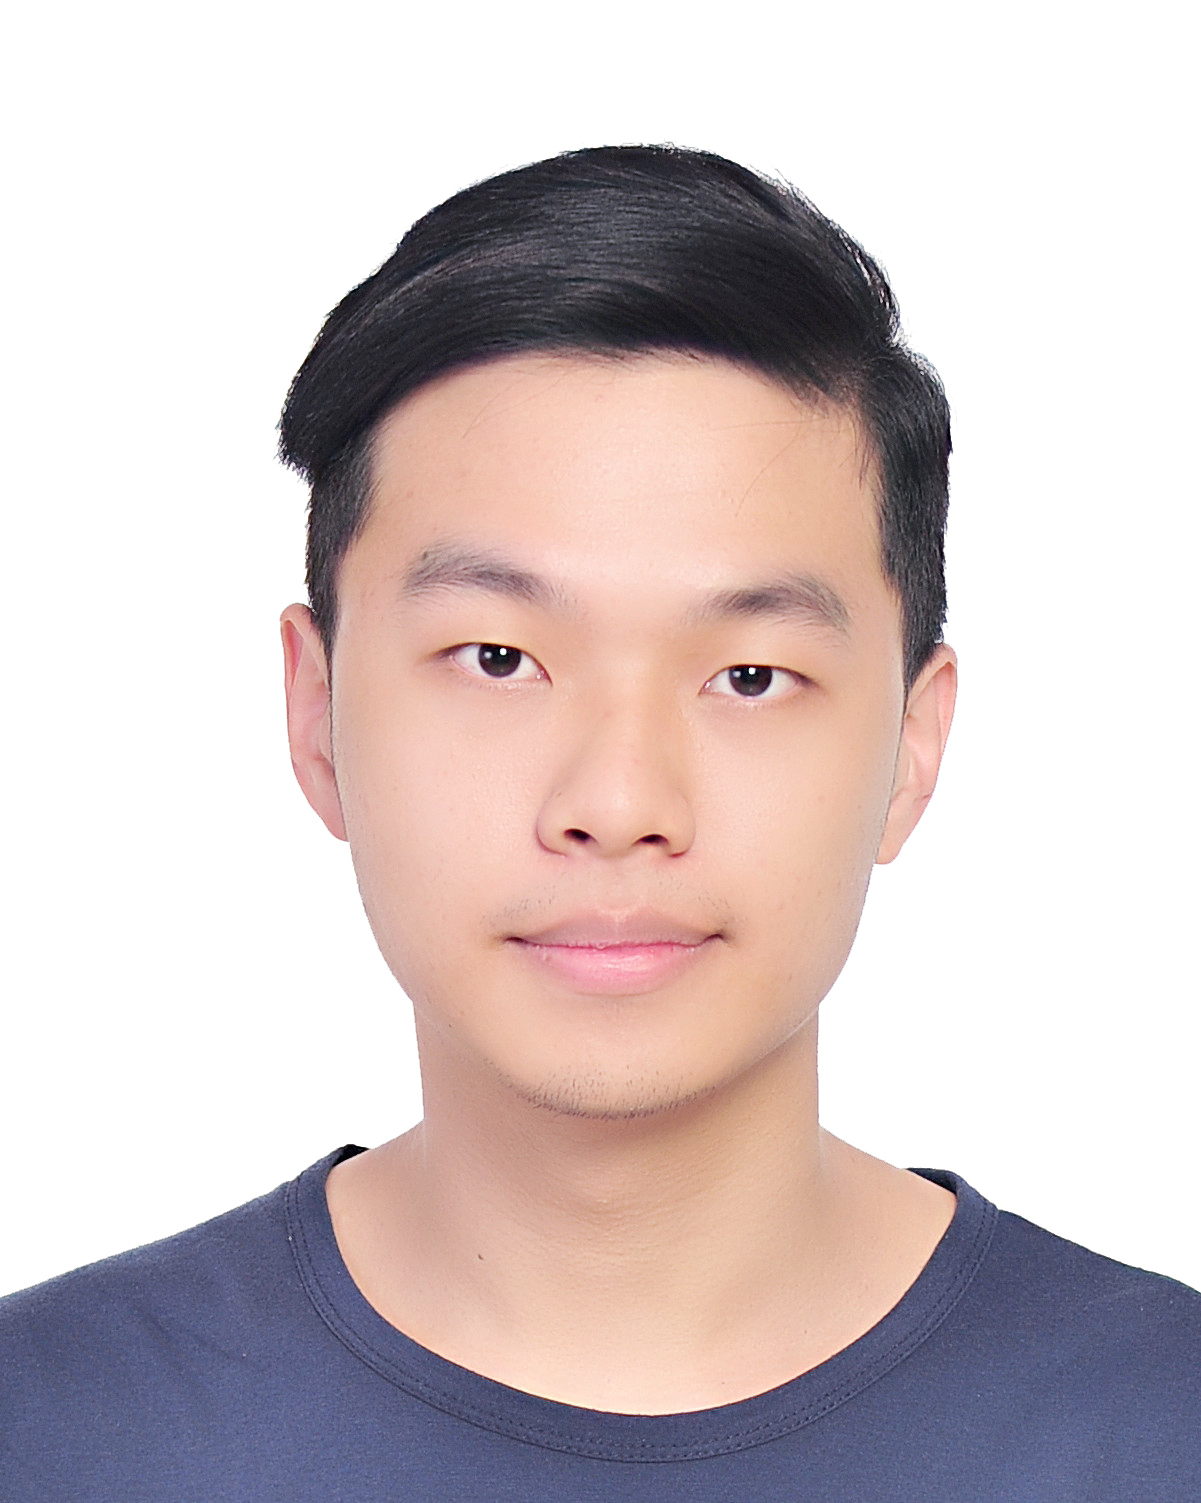
\includegraphics[width=1in,height=1.25in,clip,keepaspectratio]{./avatars/chia-chi.jpg}}]
{Chia-Chi Chen} was born in 1994 and  received the B.S. degree in Computer Science in 2016 from National Tsing Hua University, Taiwan.
He is a graduate student and major in Computer Science from National Tsing Hua University now.
Mr. Chen research chiefly focuses on Software Defined Network in High Speed Network Lab at National Tsing Hua University.
\end{IEEEbiography}

\begin{IEEEbiography}
[{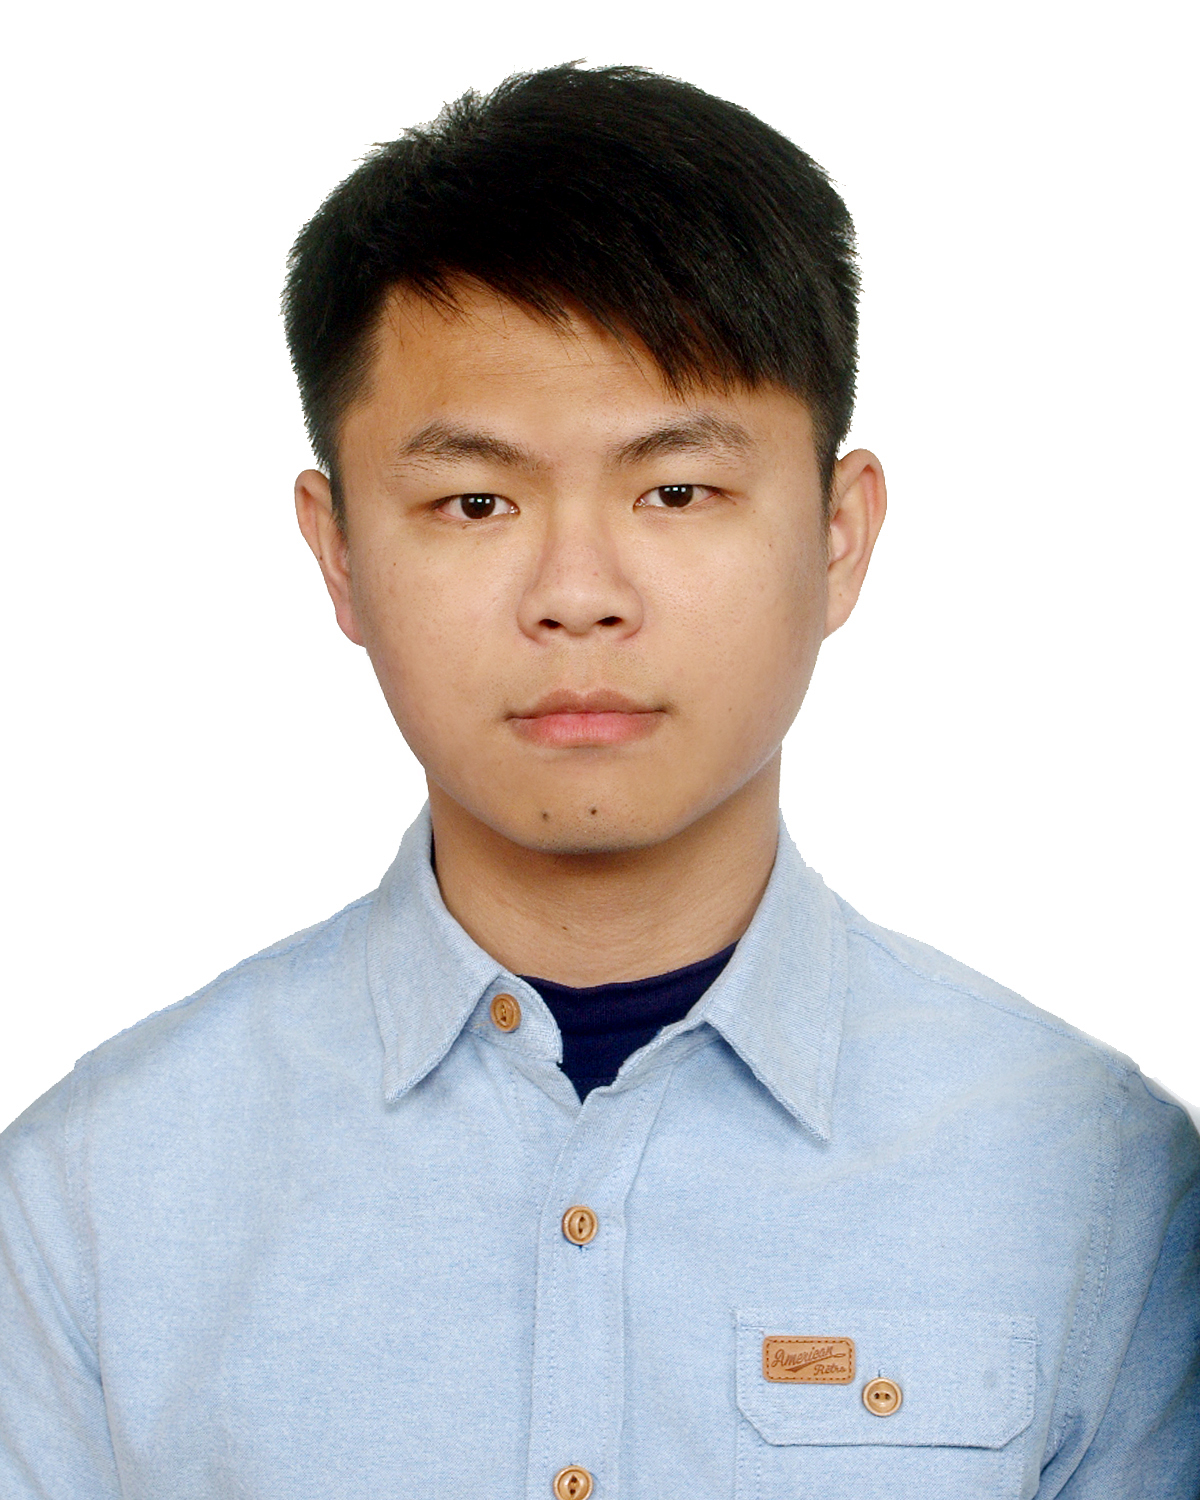
\includegraphics[width=1in,height=1.25in,clip,keepaspectratio]{./avatars/i-hsien.jpg}}]
{I-Hsien Hsu} was born in 1994 and  received the B.S. degree in Computer Science in 2016 from National Tsing Hua University, Taiwan.
He is a graduate student and major in Computer Science from National Tsing Hua University now. His research mainly focuses on Software Defined Network in High Speed Network Lab at National Tsing Hua University.
\end{IEEEbiography}

\begin{IEEEbiography}
[{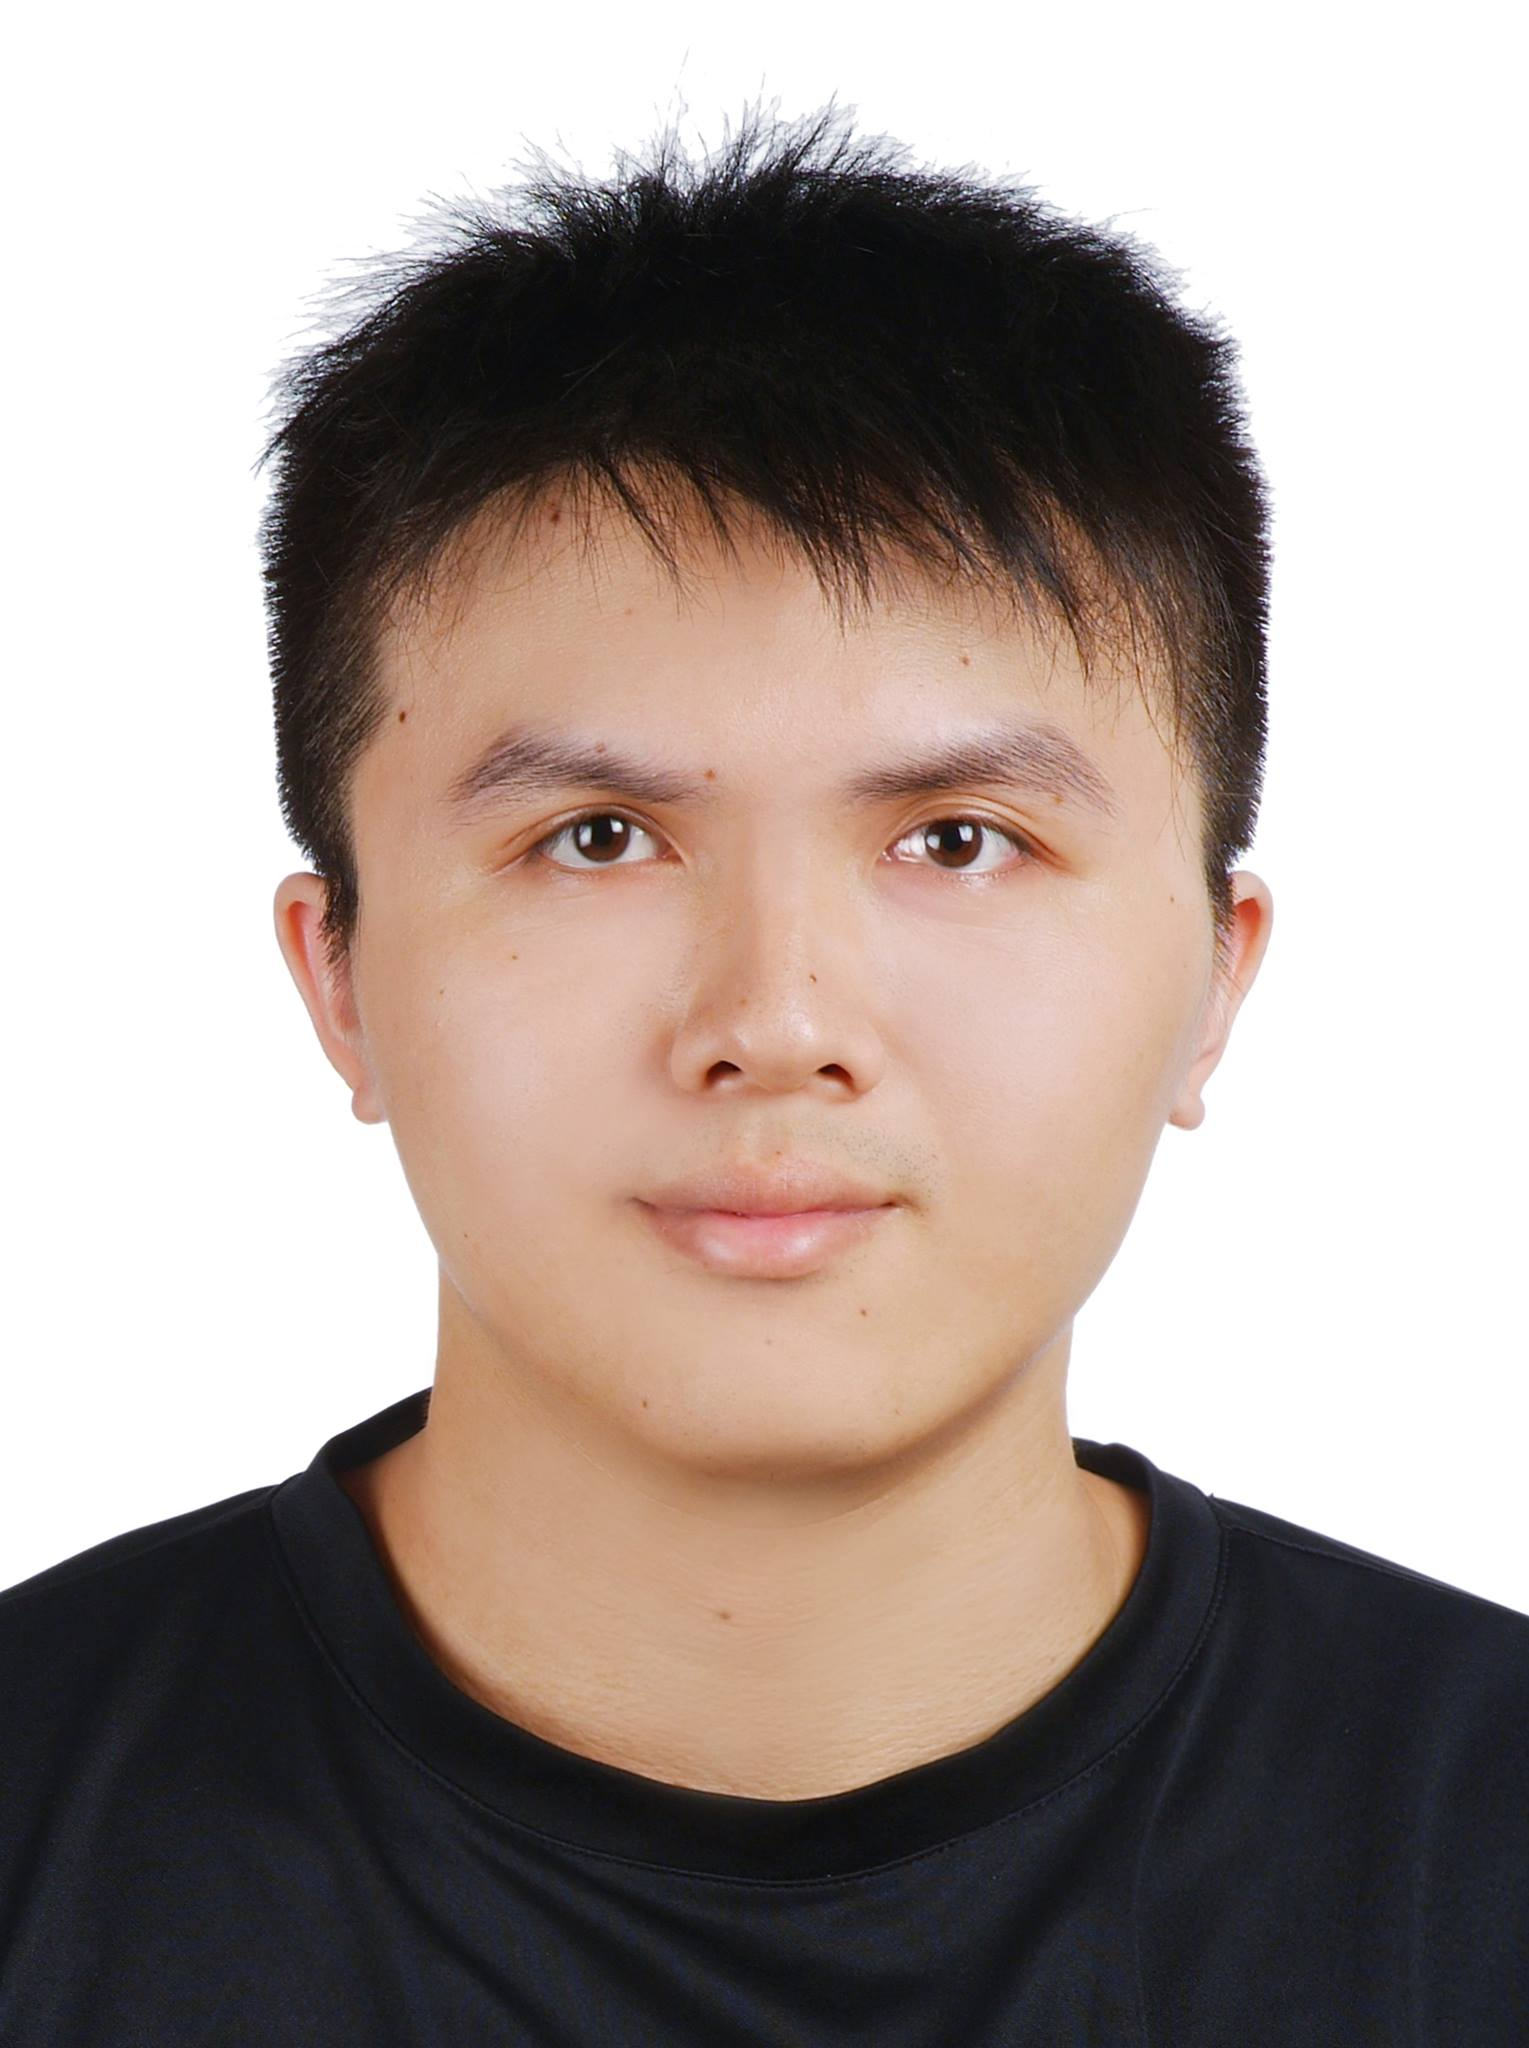
\includegraphics[width=1in,height=1.25in,clip,keepaspectratio]{./avatars/che-chuan.jpg}}]
{Che-Chuan Li} was born in Tainan City, Taiwan, in 1993. He received the B.S. degree in computer science from National Tsing Hua University, Hsinchu, Taiwan, in 2015. He is currently pursuing the M.S. degree in computer science at National Tsing Hua University, Hsinchu, Taiwan.
\end{IEEEbiography}

\begin{IEEEbiography}
[{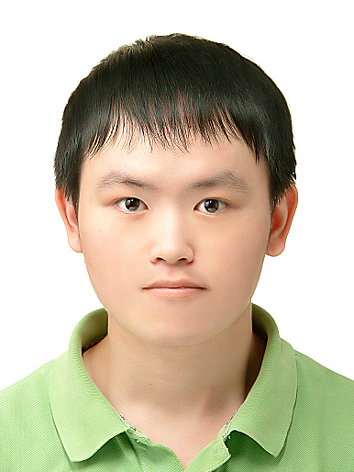
\includegraphics[width=1in,height=1.25in,clip,keepaspectratio]{./avatars/chin-hsuan.jpg}}]
{Ching-Hsuan Chen} received the bachelor degree in Computer Science department in 2016 from National Tsing Hua University, Hsinchu, Taiwan. Now he is a graduate student of the Institute of Communications Engineering in the same university, National Tsing Hua University. His research mainly focuses on Software Define Network and Network Function Virtualization.
\end{IEEEbiography}

\begin{IEEEbiography}
{I-Ju Liao}
\end{IEEEbiography}

\end{document}
